\chapter{Технологический раздел}
\label{cha:impl}

В данноой части работы выполняется разработка приложения и дается описание презентационного уровня приложения.

\section{Выбор и обоснование языка программирования и среды разработки}

\begin{itemize}
    \item Генератор данных: Python, Faker (пакет генерирует данные)
    \item Бэкэнд: Go, Gin (http веб-фреймворк), Viper (конфигурация Go), Jwt-go (реализация Golang json web token)
    \item Фронтэнд: Javascript, VueJs (прогрессивный фреймворк ), Vuex, Vue router, ElementPlus (библиотека компонентов для Vue), Axios (http-клиент на основе Promise)
    \item Редактор: VSCode, Jupyter Lab
\end{itemize}

Для взаимодействия с базой данных в этой работе я построю одностраничное веб-приложение, оно будет делать вызовы api на сервер, сервер взаимодействует с базой данных и обрабатывает данные, возвращая их клиенту.

\subsection*{Gin}

Gin - это веб-фреймворк HTTP, написанный на Go (Golang).
Этот фреймворк имеет очень хорошую производительность, в настоящее время имеет 48,7 тыс. эвезд на github, с довольно полным набором инструментов.
Go - компилируемый многопоточный язык программирования, разработанный внутри компании Google.
Поскольку это скомпилированный высокопроизводительный язык, я предпочитаю его Python, хотя у меня больше опыта работы с Python и знакомы с Flask и Django.

\subsection*{VueJs}

Веб-приложение для социальных сетей, увлекательное и очень интерактивное, с приятным интерфейсом это необходимо, или, по крайней мере, он должен быть простым в использовании.
Vue - прогрессивный фреймворк для создания пользовательских интерфейсов.
В отличие от фреймворков-монолитов, Vue создавался пригодным для постепенного внедрения. Его ядро в первую очередь решает задачи уровня представления (view), упрощая интеграцию с другими библиотеками и существующими проектами.
С другой стороны, Vue полностью подходит и для разработки сложных одностраничных приложений (SPA, Single-Page Applications), если использовать его в комбинации с современными инструментами и дополнительными библиотеками.


Учитывая объем кода, который можно назвать довольно большим (более 80 файлов исходного кода), перечислены только те компоненты, которые считаны важными.


\section{Генератор данных}

Генератор написан на python, имеет 8 классов для представления 8 таблиц, класс User для представления действий пользователя и класс Network для представления смоделированного поведения пользователей в сети во времени.
Логика генератора: генерировать соль и хэш для паролей, фотки случайным образом берутся с существующих серверов, пользователи комментируют сообщения друзей, пользователи больше взаимодействуют с новыми сообщениями, количество пользователей и количество взаимодействий со временем увеличиваются.
Созданные учетные записи также имеют резервные копии паролей для целей отладки.
Хороший генератор генерирует хороший набор данных, что очень важно при работе с базами данных.


\section{Бэкэнд}

\subsection*{Модель предметной области}

\lstinputlisting[language=Go,linerange={0-200},caption=Модель предметной области]{code/model.go}
\vbox{}

\subsection*{Компонент доступа к данным}

\lstinputlisting[language=Go,linerange={0-200},caption=Интерфейс компонента доступа к данным]{code/repo.go}
\vbox{}

\subsection*{Контроллер}

\lstinputlisting[language=Go,tabsize=2,linerange={0-200},caption=Маршрутизатор контроллера]{code/router.go}
\vbox{}


\section{Фронтэнд}

\lstinputlisting[language=javascript,linerange={0-200},caption=Маршрутизатор]{code/router.js}
\vbox{}
\pagebreak
\lstinputlisting[language=javascript,linerange={0-200},caption=модуль выполняет вызов API для компонента Post]{code/post.js}
\vbox{}


\section{Интерфейс программы}


\begin{figure}[H]
    \centering
    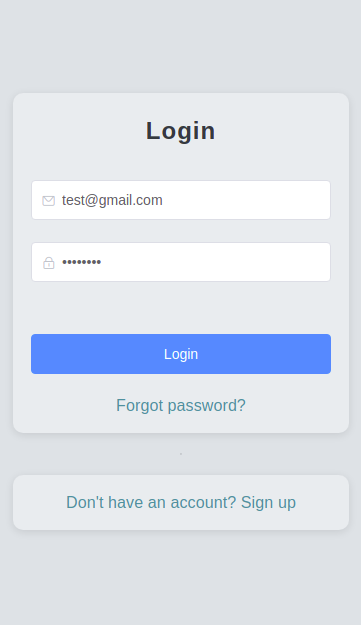
\includegraphics[width=0.4\textwidth]{img/login.png}
    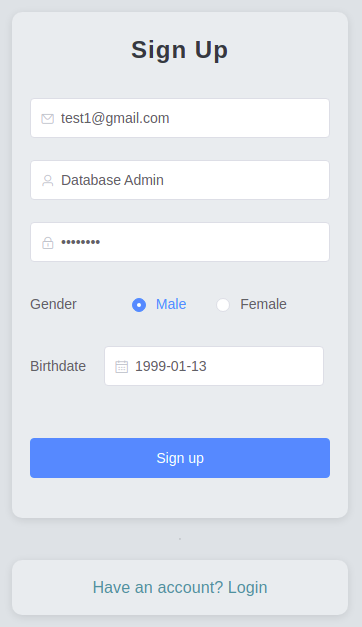
\includegraphics[width=0.4\textwidth]{img/signup.png}
    \caption{Функция входа, функция регистрации}
\end{figure}

\begin{figure}[H]
    \centering
    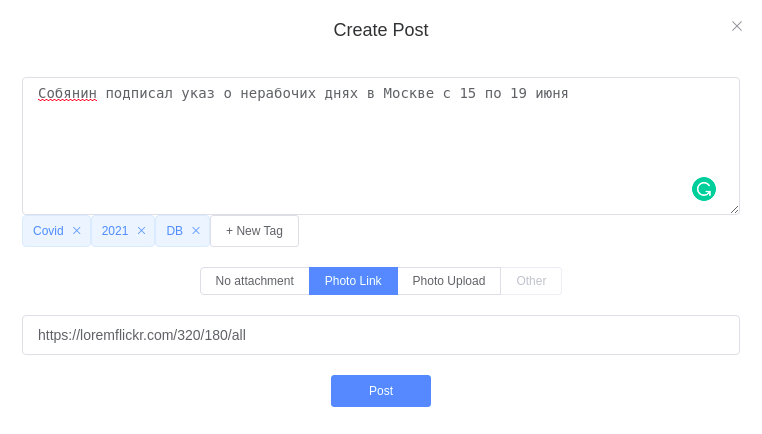
\includegraphics[width=\textwidth]{img/post.png}
    % 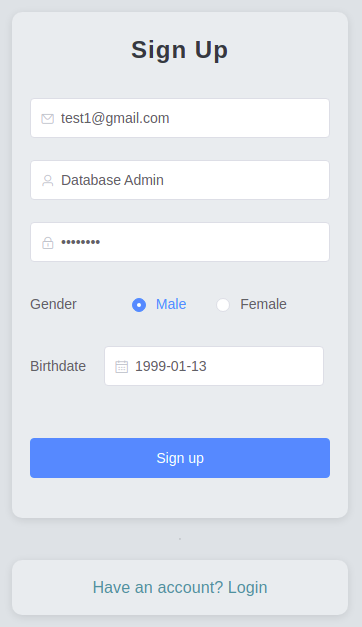
\includegraphics[width=0.48\textwidth]{img/signup.png}
    \caption{Функция публикации}
\end{figure}

\begin{figure}[H]
    \centering
    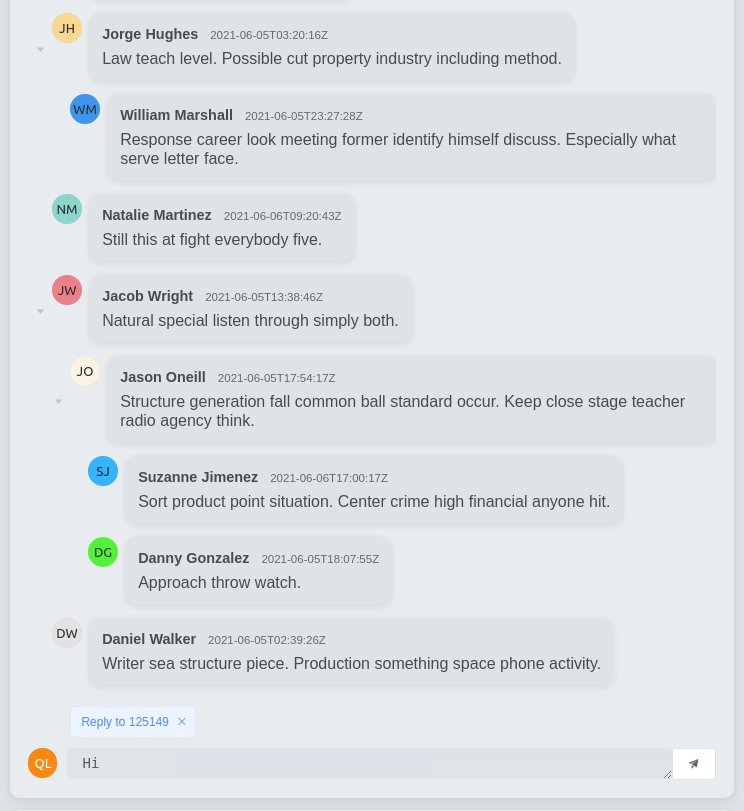
\includegraphics[width=0.9\textwidth]{img/cmt.png}
    \caption{Функция комментирования}
\end{figure}

\begin{figure}[H]
    \centering
    
\includegraphics[width=0.9\textwidth]{img/react.png}
    \caption{Функция реагирования}
\end{figure}

\begin{figure}[H]
    \centering
    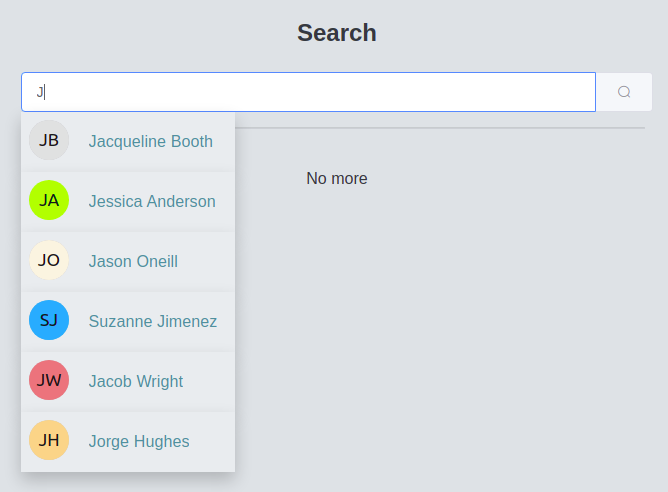
\includegraphics[width=0.7\textwidth]{img/search1.png}
    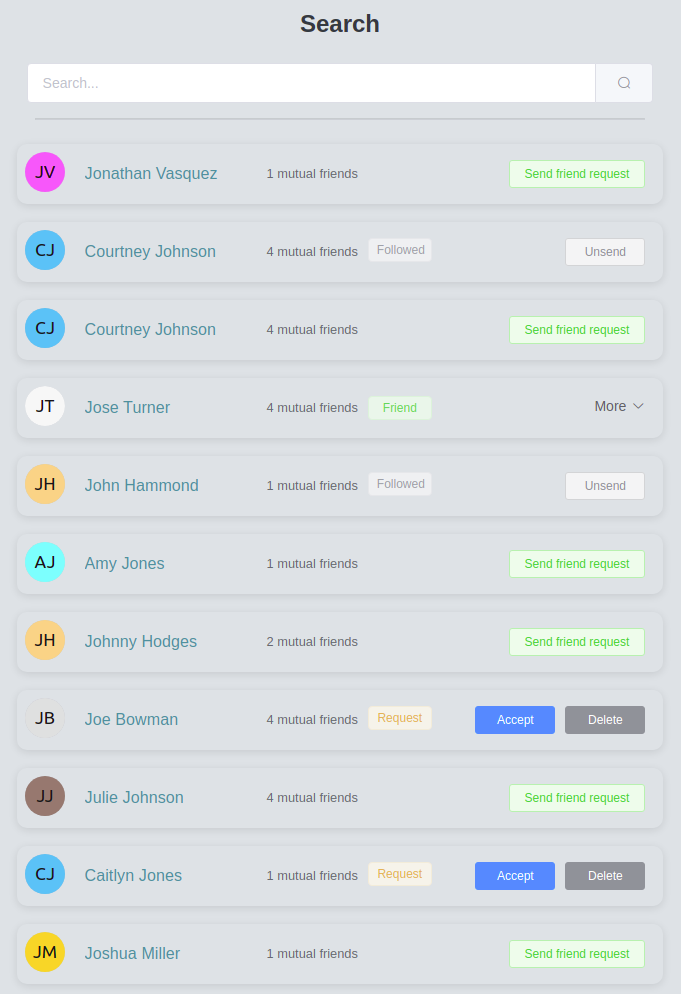
\includegraphics[width=0.7\textwidth]{img/search2.png}
    \caption{Функция поиска по имени пользователя}
\end{figure}

\begin{figure}[H]
    \centering
    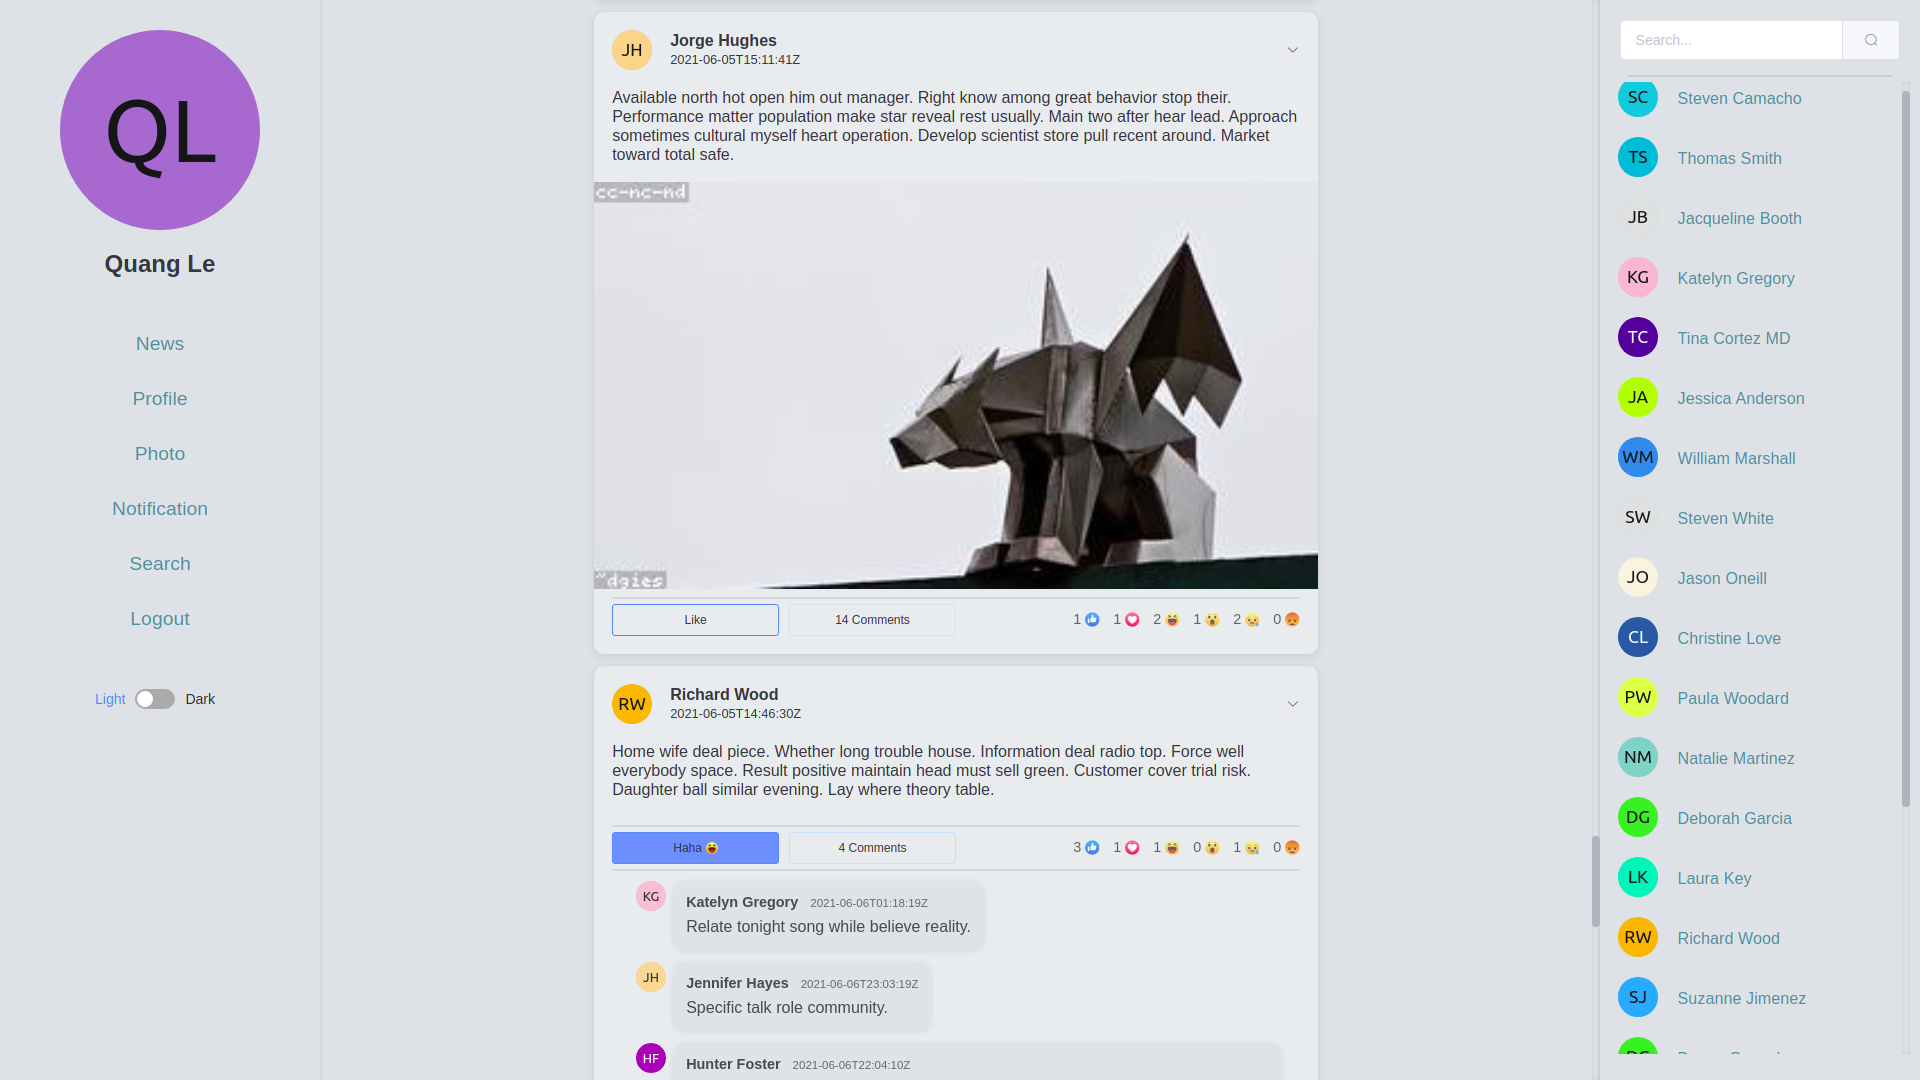
\includegraphics[width=\textwidth]{img/feed.png}
    \caption{Страница новостей}
\end{figure}

\begin{figure}[H]
    \centering
    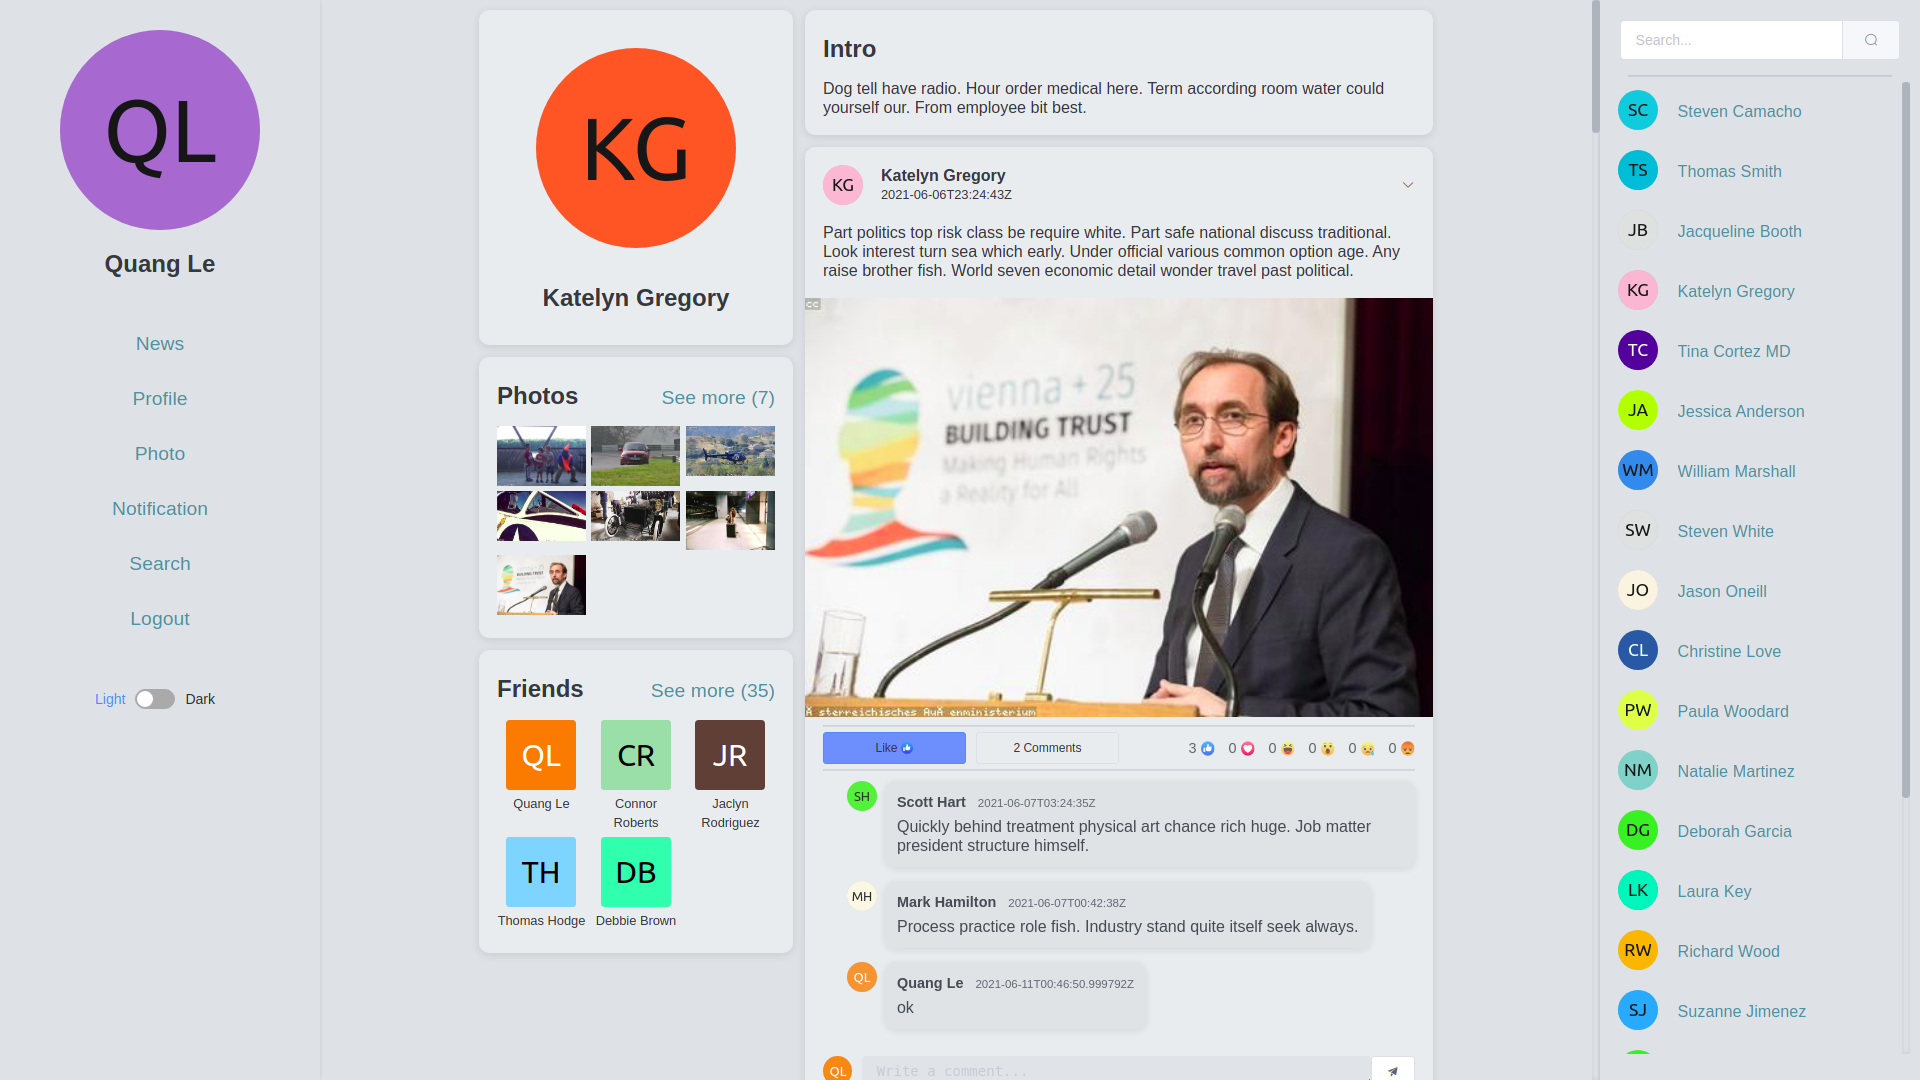
\includegraphics[width=\textwidth]{img/profile.png}
    \caption{Страница профиля}
\end{figure}

\section*{Вывод}

Были рассмотрено описание генератора данных, а также перечислены некоторые важные коды серверной части и клиентской части.